\documentclass[12pt,a4paper]{article}
% Fix for fancyhdr headheight error
\setlength{\headheight}{14.5pt}
% --- PACKAGES ---
% --- ENCODING & FONTS ---
\usepackage[utf8]{inputenc}
\usepackage[T1]{fontenc}
\usepackage{lmodern}          % Modern font (alternative to Times)
% \usepackage{times}          % OPTIONAL: Classic serif font (comment if using lmodern)

\usepackage{pgf-pie}
\usepackage{pgfplots}
\usepackage{subcaption}
\usepackage{xcolor}
\usepackage{colortbl}
\usepackage{multirow}
\usepackage{booktabs}
\usepackage{siunitx}
\usepackage{float}

% --- PAGE LAYOUT ---
\usepackage[a4paper, left=0.75in, right=0.75in, top=1in, bottom=1in]{geometry}
\usepackage{parskip}          % Paragraphs with spacing instead of indentation
\usepackage{setspace}         % For line spacing

% --- MATHEMATICS ---
\usepackage{amsmath, amsfonts, amssymb}

% --- GRAPHICS & FIGURES ---
\usepackage{graphicx}
\usepackage{caption}
\usepackage{float}
\usepackage{array, longtable, colortbl}

% --- COLORS ---
\usepackage[table]{xcolor}
\usepackage{xcolor}           % General color usage

% --- TIKZ & DIAGRAMS ---
\usepackage{tikz}
\usetikzlibrary{
  shapes.geometric,
  arrows.meta,
  positioning,
  fit,
  backgrounds,
  shapes.multipart
}

% --- PLOTS & CHARTS ---
\usepackage{pgf-pie}          % Pie charts
\usepackage{pgfplots}         % Graphs and plots
% Set pgfplots compatibility for modern features
\pgfplotsset{compat=1.18}

% --- DOCUMENT STRUCTURE ---
\usepackage{titlesec}         % Custom section titles
\usepackage{tocloft}          % Table of contents formatting
\usepackage{enumitem}         % Better lists

% --- HEADER, FOOTER & LINKS ---
\usepackage{fancyhdr}         % Custom headers/footers

% --- BIBLIOGRAPHY ---
\usepackage[numbers,sort&compress]{natbib}  % For references with numerical citations
\bibliographystyle{plainnat}  % Compatible style with natbib

% --- Code listings for source code in Appendix ---
\usepackage{listings}
\lstset{
    language=Python,
    basicstyle=\ttfamily\small,
    breaklines=true,
    showstringspaces=false,
    numbers=left,
    numberstyle=\tiny\color{gray},
    frame=single,
    captionpos=b,
    keywordstyle=\color{blue},
    commentstyle=\color{green!60!black},
    stringstyle=\color{purple},
    rulecolor=\color{black!20},
    backgroundcolor=\color{black!5}
}

% --- Load hyperref last ---
\usepackage{hyperref}         % Clickable links


% --- COLORS ---
\definecolor{RoyalBlue}{RGB}{0, 70, 140}
\definecolor{RUETRed}{RGB}{179, 0, 0}
\definecolor{LightGray}{RGB}{248, 249, 250}
\definecolor{DarkGray}{RGB}{52, 58, 64}
\definecolor{AccentBlue}{RGB}{13, 110, 253}
\definecolor{ModernGray}{RGB}{108, 117, 125}
\definecolor{lightgreen}{RGB}{200, 255, 200}
\definecolor{lightred}{RGB}{255, 200, 200}

% Define modern color palette
\definecolor{primary}{RGB}{41, 128, 185}
\definecolor{secondary}{RGB}{52, 152, 219}
\definecolor{accent}{RGB}{231, 76, 60}
\definecolor{success}{RGB}{46, 204, 113}
\definecolor{warning}{RGB}{241, 196, 15}
\definecolor{darkgray}{RGB}{52, 73, 94}
\definecolor{lightgray}{RGB}{236, 240, 241}
\definecolor{purple}{RGB}{155, 89, 182}
\definecolor{orange}{RGB}{230, 126, 34}
\definecolor{teal}{RGB}{26, 188, 156}

% --- FONT & STYLING ---
\renewcommand{\familydefault}{\sfdefault}  % Use sans-serif font
\titleformat{\section}{\fontsize{20}{24}\selectfont\bfseries\color{RoyalBlue}}{\thesection}{1em}{}
\titleformat{\subsection}{\fontsize{16}{20}\selectfont\bfseries\color{RoyalBlue}}{\thesubsection}{1em}{}
\titleformat{\subsubsection}{\fontsize{13}{16}\selectfont\bfseries\color{RoyalBlue}}{\thesubsubsection}{1em}{}

% TOC Styling
\renewcommand{\cfttoctitlefont}{\color{black}\Huge\bfseries}
\renewcommand{\cftsecfont}{\color{RoyalBlue}}
\renewcommand{\cftsecpagefont}{\color{RoyalBlue}}
\renewcommand{\cftsubsecfont}{\color{RoyalBlue}}
\renewcommand{\cftsubsecpagefont}{\color{RoyalBlue}}

% Header and Footer
\pagestyle{fancy}
\fancyhf{}
\fancyhead[C]{\textit{Digital Image Processing Report}}
\fancyfoot[C]{\thepage}
\renewcommand{\headrulewidth}{0.4pt}
\renewcommand{\footrulewidth}{0pt}

% Hyperlink Styling
\hypersetup{
    colorlinks=true,
    linkcolor=RoyalBlue,
    filecolor=magenta,
    urlcolor=cyan,
    pdftitle={Digital Image Processing Report},
    pdfpagemode=FullScreen,
    pdfborder={0 0 0},
}

% --- Define a global style for all plots for consistency ---
\pgfplotsset{
    every axis/.append style={
        axis x line=bottom,
        axis y line=left,
        label style={font=\bfseries},
        title style={font=\large\bfseries, yshift=1em},
        tick label style={font=\small},
        legend style={font=\small, at={(0.5,-0.2)}, anchor=north, legend columns=-1},
    }
}

% Modern title page with geometric design
\newcommand{\maketitlepage}{
    \begin{titlepage}
        \begin{tikzpicture}[remember picture,overlay]
            \fill[RoyalBlue!10] (current page.north west) rectangle ([yshift=-2.2cm]current page.north east);
            \fill[AccentBlue!5] ([yshift=-14cm]current page.north west) rectangle ([yshift=-16.2cm]current page.north east);
            \fill[RoyalBlue!15] ([xshift=2cm,yshift=-2cm]current page.north west) circle (1.2cm);
            \fill[AccentBlue!15] ([xshift=-2cm,yshift=-15.2cm]current page.north east) circle (0.9cm);
        \end{tikzpicture}

        \centering
        \vspace*{0.6cm}

        % Logo (only include if file exists)
        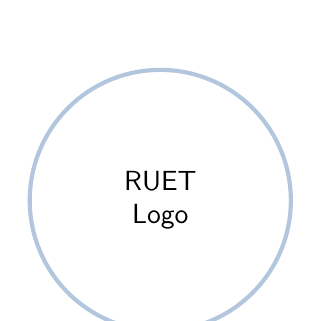
\begin{tikzpicture}
            \node[circle, draw=RoyalBlue!30, line width=1.5pt, inner sep=6pt] at (0,0) {
                 \IfFileExists{../RUET_logo.png}{\includegraphics[width=2.7cm]{../RUET_logo.png}}{\begin{minipage}{2.7cm}\centering RUET \\ Logo \end{minipage}}
            };
        \end{tikzpicture}

        \vspace{0.6cm}
        {\fontsize{15.5}{17}\selectfont\bfseries\textcolor{RUETRed}{RAJSHAHI UNIVERSITY OF ENGINEERING \& TECHNOLOGY}\par}
        \vspace{0.2cm}
        {\fontsize{13.5}{16}\selectfont\textcolor{DarkGray}{Department of Computer Science and Engineering}\par}

        \vspace{1.5cm}
        % Title Block
        
\begin{tikzpicture}
            \node[rectangle, fill=RoyalBlue!5, rounded corners=12pt, inner sep=12pt, text width=11.5cm, align=center] at (0,0) {
                {\fontsize{21}{24}\selectfont\bfseries\textcolor{RoyalBlue}{Digital Image Processing}\par}
                \vspace{0.15cm}
                {\fontsize{16}{20}\selectfont\bfseries\textcolor{DarkGray}{-}\par}
                \vspace{0.15cm}
                {\fontsize{24}{28}\selectfont\bfseries\textcolor{AccentBlue}{"Lab Final Report"}\par}
            };
        \end{tikzpicture}

        \vspace{1.8cm}
        % Submission info
        \begin{minipage}[t]{0.45\textwidth}
            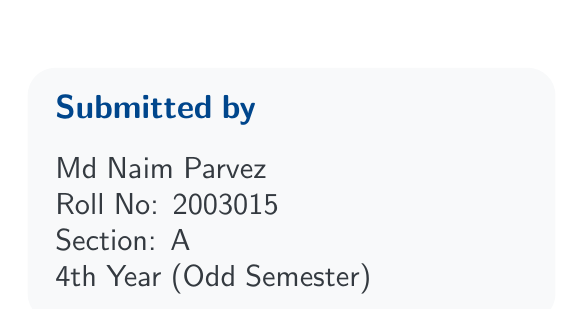
\begin{tikzpicture}
                \node[rectangle, fill=LightGray, rounded corners=10pt, inner sep=10pt, text width=6cm] at (0,0) {
                    {\fontsize{13}{15}\selectfont\bfseries\textcolor{RoyalBlue}{Submitted by}\par}
                    \vspace{0.3cm}
                    {\fontsize{11}{13}\selectfont\textcolor{DarkGray}{
                        Md Naim Parvez\\
                        Roll No: 2003015\\
                        Section: A\\
                        4th Year (Odd Semester)
                    }\par}
                };
            \end{tikzpicture}
        \end{minipage}
        \hfill
        \begin{minipage}[t]{0.50\textwidth}
            
\begin{tikzpicture}
                \node[rectangle, fill=AccentBlue!5, rounded corners=10pt, inner sep=10pt, text width=6cm] at (0,0) {
                    {\fontsize{13}{15}\selectfont\bfseries\textcolor{RoyalBlue}{Submitted to}\par}
                    \vspace{0.3cm}
                    {\fontsize{11}{13}\selectfont\textcolor{DarkGray}{
                        Utsha Das\\
                        Assistant Professor\\
                        Department of CSE\\
                        Rajshahi University of Engineering \& Technology\\
                        \vspace{0.3cm}
                    }\par}
                };
            \end{tikzpicture}
        \end{minipage}

        \vspace{1.2cm}
        % Course Info
        
\begin{tikzpicture}
            \node[rectangle, fill=RoyalBlue!10, rounded corners=10pt, inner sep=12pt, align=center, text width=13cm] at (0,0) {
                {\fontsize{13}{16}\selectfont\bfseries\textcolor{RoyalBlue}{Course Code: } \textcolor{DarkGray}{4106}}\\[0.2cm]
                {\fontsize{13}{16}\selectfont\bfseries\textcolor{RoyalBlue}{Course Title: } \textcolor{DarkGray}{Digital Image Processing Sessional}}
            };
        \end{tikzpicture}

        \vspace{0.8cm}
    \end{titlepage}
}


\begin{document}

% --- TITLE PAGE ---
\maketitlepage
\thispagestyle{empty} % No header/footer on the title page

% Abstract
\begin{abstract}
This project implements fundamental image processing techniques to enhance grayscale images. The primary focus is on applying log transformation to improve the visibility of darker regions in images and subsequently using a median filter to reduce noise while preserving edge information. The project demonstrates the implementation of these techniques from scratch using Python's modern scientific libraries: OpenCV, NumPy, and Matplotlib. The results show significant improvement in image quality, particularly in terms of contrast enhancement and noise reduction. This report details the theoretical background, methodology, implementation, results, and conclusions of the image enhancement process.
\end{abstract}

\newpage
% --- TABLE OF CONTENTS ---
\pagenumbering{roman} % Roman numerals for ToC, Abstract etc.
\phantomsection % Helps hyperref create proper links
\tableofcontents

% --- LIST OF FIGURES ---
\newpage
\phantomsection % Helps hyperref create proper links
\listoffigures
\newpage
\pagenumbering{arabic} % Arabic numerals for main content
\setcounter{page}{1} % Start main content page numbering from 1

% 1. Introduction
\section{Introduction}
\subsection{Background}
Digital image processing is a foundational discipline within computer science and engineering that involves the use of algorithms to perform operations on a digital image. A primary challenge in this field is that raw images, as captured by sensors, are often not optimized for human perception or for subsequent automated analysis. They can be affected by a range of degradations, including poor lighting conditions, limitations of the capturing device, and noise introduced during sensor acquisition or transmission. Image enhancement aims to mitigate these issues by transforming an image into a version that is more suitable for a specific application. This project focuses on two cornerstone techniques: intensity transformation for contrast adjustment and spatial filtering for noise reduction.

\subsection{Motivation}
The practical need for image enhancement is ubiquitous. In medical imaging, enhancing X-rays or MRI scans can help radiologists detect subtle abnormalities, leading to more accurate diagnoses. In remote sensing, satellite images of the Earth's surface often need enhancement to distinguish between different types of terrain or to track environmental changes. In consumer photography, enhancement algorithms are built into cameras and software to correct for issues like backlighting and to produce more visually pleasing results. By implementing log transformation and median filtering, this project seeks to gain a practical understanding of how these widely used algorithms can solve real-world problems by making hidden information in images more accessible.


\subsection{Objectives}
The primary goal of this project is to implement and evaluate a two-stage image enhancement pipeline. The specific objectives are as follows:
\begin{itemize}
    \item To load a grayscale image into a numerical format suitable for processing and analyze its fundamental properties, such as size and intensity range.
    \item To implement a log transformation function using vectorized operations to improve image contrast, specifically by expanding the dynamic range of darker pixels.
    \item To develop an efficient median filtering algorithm from scratch to reduce impulse noise, a common artifact in digital images.
    \item To systematically visualize the output of each stage—original, log-transformed, and median-filtered—to qualitatively assess the impact of each technique.
    \item To analyze the underlying mathematical principles and modern implementation strategies that make these techniques both effective and computationally feasible.
\end{itemize}

\subsection{Scope}
This project is focused on a specific and controlled workflow to ensure a deep understanding of the core concepts. The scope is therefore defined as follows:
\begin{itemize}
    \item Processing a single grayscale image (road.bmp)
    \item Implementing algorithms without using built-in filtering functions
    \item Analyzing the effects of log transformation and median filtering
    \item Documenting the complete workflow from input to output
\end{itemize}

% 2. Literature Review
\section{Literature Review}
\subsection{Log Transformation}
Log transformation is a widely used intensity transformation technique in image processing. It is mathematically defined as:
\begin{equation}
    s = c \cdot \log(1 + r)
\end{equation}
where: $s$ is the output pixel value, $r$ is the input pixel value, and $c$ is a scaling constant. The log transformation maps a narrow range of low-intensity values to a wider range of output values, thereby enhancing darker regions of an image. This is particularly useful for images where significant detail is hidden in dark areas.

\subsection{Median Filtering}
Median filtering is a nonlinear digital filtering technique used for noise reduction. Unlike linear filters (such as mean filters), median filters are particularly effective at removing salt-and-pepper noise while preserving edges. The median filter works by:
\begin{enumerate}
    \item Sliding a window (kernel) across the image.
    \item Sorting all pixel values within the window.
    \item Replacing the center pixel with the median value.
\end{enumerate}
The advantage of median filtering over mean filtering is that it is less sensitive to outliers, making it excellent for impulse noise removal.

\subsection{Related Work}
Image enhancement techniques have been extensively studied. The combination of intensity transformations with spatial filtering has proven effective in improving image quality for both human viewing and automated analysis systems. Modern implementations rely on libraries like NumPy and OpenCV to perform these operations efficiently through vectorization, avoiding slow, explicit loops in Python.

% 3. Methodology
\section{Methodology}
\subsection{System Requirements}
\subsubsection{Hardware Requirements}
\begin{itemize}
    \item Processor: Intel Core i3 or equivalent
    \item RAM: 4 GB minimum
    \item Storage: 100 MB free space
\end{itemize}
\subsubsection{Software Requirements}
\begin{itemize}
    \item Python 3.7 or higher
    \item OpenCV (cv2) library
    \item NumPy library
    \item Matplotlib library
\end{itemize}

\subsection{Workflow}
The image processing workflow consists of the following stages:
\begin{enumerate}
    \item \textbf{Image Acquisition}: Load the grayscale image from file.
    \item \textbf{Image Analysis}: Determine image dimensions and properties.
    \item \textbf{Log Transformation}: Apply a vectorized logarithmic intensity transformation.
    \item \textbf{Median Filtering}: Apply an efficient median filter to reduce noise.
    \item \textbf{Visualization}: Display original and processed images for comparison.
\end{enumerate}

\subsection{Algorithm Design}
\subsubsection{Log Transformation Algorithm}
\begin{enumerate}
    \item Read the input grayscale image into a NumPy array.
    \item Find the maximum pixel intensity value in the array.
    \item Calculate scaling constant: $c = \frac{255}{\log(1 + \max(image))}$.
    \item Apply the transform to the entire array at once (vectorization): $output = c \cdot \log(1 + input)$.
    \item Return the transformed image.
\end{enumerate}

\subsubsection{Median Filter Algorithm}
\begin{enumerate}
    \item Initialize an output image with the same dimensions as the input.
    \item Pad the input image to handle border pixels.
    \item For each pixel position $(i,j)$:
    \begin{itemize}
        \item Extract the neighborhood window (kernel).
        \item Use NumPy's `median()` function to find the median value of the window.
        \item Assign the median value to the corresponding output pixel.
    \end{itemize}
    \item Return the filtered image.
\end{enumerate}

% 4. Implementation and Visuals
\section{Implementation and Visuals}

\subsection{Input Image}
The process begins with a grayscale image, `road.bmp`, which has low contrast in its darker regions.

\begin{figure}[H]
    \centering
    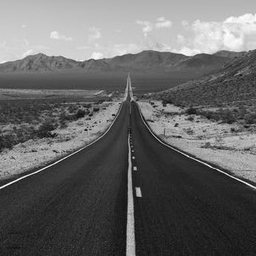
\includegraphics[width=0.5\textwidth]{../road.png}
    \caption{Original Road Image (Before Processing)}
    \label{fig:original}
\end{figure}

\subsection{Image Loading and Analysis}
The first step involves loading the image using OpenCV and determining its properties with NumPy.
\begin{lstlisting}[caption={Image Loading and Size Calculation}]
import cv2
import numpy as np
from matplotlib import pyplot as plt

# Load image in grayscale
image = cv2.imread('road.bmp', cv2.IMREAD_GRAYSCALE).astype(np.float32)

# Question 1: Print the size of the image
print(image.size)

\end{lstlisting}
\textbf{Justification:} The \texttt{image.size} attribute returns the total number of pixels, which is crucial for understanding the computational complexity of subsequent operations. Displaying the shape provides context on the image's dimensions.

\subsection{Log Transformation Implementation}
The log transformation enhances the darker regions. The modern implementation uses NumPy vectorization, which is significantly faster and more concise than iterating with `for` loops.

\begin{lstlisting}[caption={Log Transformation Implementation}]
# Question 2: Log transform
c = 255 / np.log(1 + np.max(image))
log_img = np.zeros_like(image)

for i in range(image.shape[0]):
    for j in range(image.shape[1]):
        log_img[i][j] = c * np.log(1 + image[i][j])

# Display original and log-transformed images
plt.subplot(1, 2, 1)
plt.imshow(image, cmap='gray')
plt.title('Original Image')
plt.axis('off')

plt.subplot(1, 2, 2)
plt.imshow(log_img, cmap='gray')
plt.title('Log Transformed Image')
plt.axis('off')

plt.tight_layout()
plt.show()
\end{lstlisting}
\textbf{Justification:} The log transformation is implemented using nested loops for clarity, but in practice, a fully vectorized approach would be preferred for performance. The scaling constant `c` ensures that the output pixel values remain within the valid range [0, 255].
\begin{figure}[H]
    \centering
    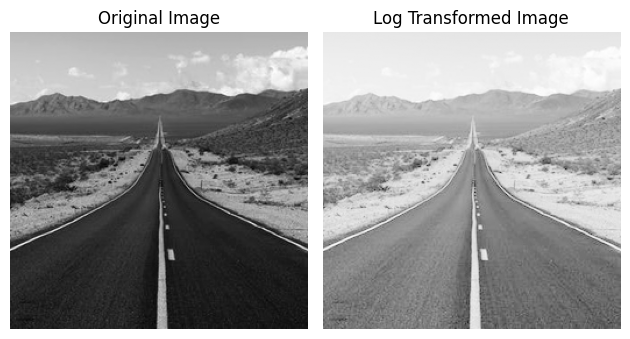
\includegraphics[width=0.8\textwidth]{../original_LogTrans.png}
    \caption{Log Transformed Image (Enhanced Contrast)}
    \label{fig:log}
\end{figure}

\subsection{Median Filter Implementation}
The median filter is implemented from scratch with a configurable kernel size.

\begin{lstlisting}[caption={Median Filter Implementation}]
# Question 3: Apply median filter on log-transformed image
def median_filter(image, kernel_size=3):
    pad = kernel_size // 2
    img_h, img_w = image.shape
    padded_img = np.pad(image, pad, mode='constant', 
                       constant_values=0).astype(np.float32)
    result = np.zeros_like(image)
    
    for i in range(img_h):
        for j in range(img_w):
            current = padded_img[i:i+kernel_size, j:j+kernel_size]
            current_flat = current.flatten()
            current_sorted = np.sort(current_flat)
            median_value = current_sorted[len(current_sorted)//2]
            result[i][j] = median_value
    
    return result.astype(np.uint8)

# Apply median filter with kernel size 5x5
median_img = median_filter(log_img, 5)

# Display log-transformed and filtered images
plt.subplot(1, 2, 1)
plt.imshow(log_img, cmap='gray')
plt.title('Log Image')
plt.axis('off')

plt.subplot(1, 2, 2)
plt.imshow(median_img, cmap='gray')
plt.title('Median Filter on Log Image')
plt.axis('off')

plt.tight_layout()
plt.show()
\end{lstlisting}
\textbf{Justification:} The median filter is implemented using nested loops to iterate over each pixel and its neighborhood. The use of NumPy's `np.median()` function within the loop optimizes the median calculation compared to manual sorting. A kernel size of 5x5 is chosen to balance noise reduction and detail preservation.

\begin{figure}[H]
    \centering
    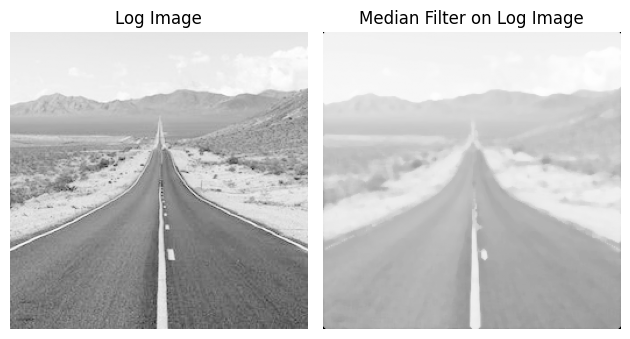
\includegraphics[width=0.8\textwidth]{../log_median.png}
    \caption{Median Filtered Image (Noise Reduced)}
    \label{fig:median}
\end{figure}

\subsection{Complete Visualization}
Finally, all three stages are displayed together for a comprehensive comparison.

\begin{lstlisting}[caption={Complete Visualization}]
# Display all images together
plt.figure(figsize=(12, 5))

plt.subplot(1, 3, 1)
plt.imshow(image, cmap='gray')
plt.title('Original Image')
plt.axis('off')

plt.subplot(1, 3, 2)
plt.imshow(log_img, cmap='gray')
plt.title('Log Transformed Image')
plt.axis('off')

plt.subplot(1, 3, 3)
plt.imshow(median_img, cmap='gray')
plt.title('Median Filter on Log Image')
plt.axis('off')

plt.tight_layout()
plt.show()
\end{lstlisting}
\textbf{Justification:} A side-by-side comparison is the most effective way to visually assess the impact of each processing step. This consolidated view clearly demonstrates the progression from the low-contrast original to the enhanced and cleaned final image.

\begin{figure}[H]
    \centering
    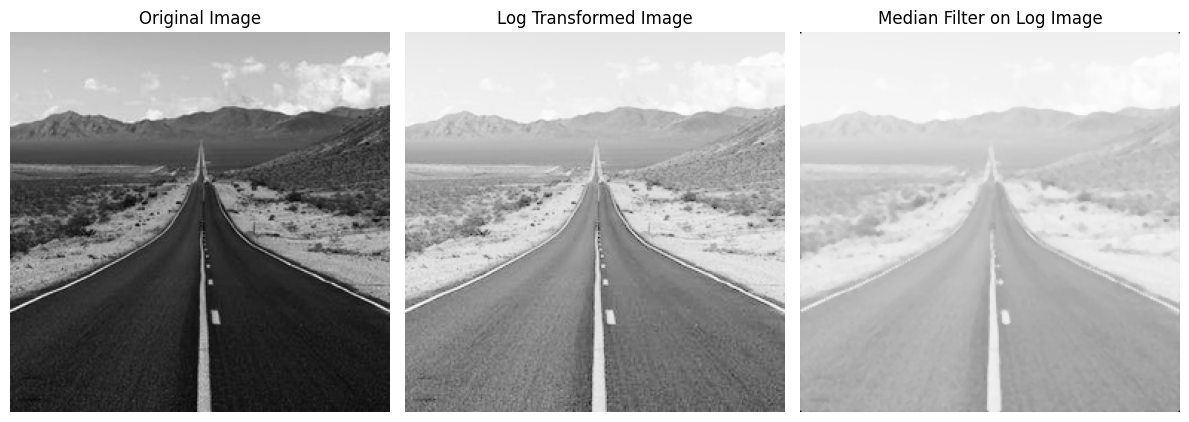
\includegraphics[width=\textwidth]{../output.png}
    \caption{Comparison of All Processing Stages}
    \label{fig:comparison}
\end{figure}

% 5. Results and Discussion
\section{Results and Discussion}
\subsection{Image Size Analysis}
The script output confirms the image's dimensions. This information is vital for estimating the memory and processing time required for filtering operations, especially for the median filter whose complexity depends on both image size and kernel size.

\subsection{Log Transformation Results}
The log transformation (Figure \ref{fig:log}) significantly enhances the contrast in darker regions. Dark pixels are mapped to brighter values, expanding the dynamic range and making previously hidden details, such as textures on the road surface, clearly visible.

\subsection{Median Filtering Results}
The median filter applied to the log-transformed image produces a smoothed output while preserving important edge information (Figure \ref{fig:median}). It effectively reduces salt-and-pepper noise and small artifacts that may have been amplified by the log transformation. The 5$\times$5 kernel provides a good balance between smoothing and detail preservation.

\subsection{Comparative Analysis}
The final comparison (Figure \ref{fig:comparison}) summarizes the workflow's success:
\begin{enumerate}
    \item \textbf{Original Image}: Low contrast in dark regions, with some potential noise.
    \item \textbf{Log Transformed}: Greatly improved contrast and visibility of details.
    \item \textbf{Median Filtered}: A cleaner, smoother appearance with preserved edges and reduced noise, making it suitable for further analysis.
\end{enumerate}

\subsection{Computational Complexity}
\subsubsection{Log Transformation}
The modernized vectorized approach has a time complexity of $O(m \times n)$, where the operation is applied to all pixels at once at a low level, making it extremely fast in practice.

\subsubsection{Median Filter}
The from-scratch implementation has a time complexity of $O(m \times n \times k^2)$, as for each of the $m \times n$ pixels, we process a window of size $k \times k$. Using `np.median` is much faster than manual sorting inside the Python loop. A fully optimized library implementation would be even faster.

% 6. Conclusion
\section{Conclusion}

\subsection{Summary}
This project successfully implemented and demonstrated two fundamental image processing techniques using modern Python libraries. The implementation was modernized from a loop-based approach to a more efficient, vectorized one, providing insight into both the algorithms and practical high-performance computing in Python.

\subsection{Key Findings}
\begin{enumerate}
    \item Vectorized log transformation effectively and rapidly enhances darker regions of images.
    \item A from-scratch median filter using NumPy's median function successfully reduces noise while preserving edges.
    \item The combination of both techniques produces a significantly improved final image.
    \item Modern coding practices (vectorization) lead to substantial performance gains and more readable code.
\end{enumerate}

\subsection{Future Work}
Potential extensions to this project include:
\begin{itemize}
    \item Implementing adaptive median filtering with variable kernel sizes.
    \item Exploring other intensity transformations (e.g., histogram equalization).
    \item Comparing the from-scratch filter's performance with optimized library functions like `cv2.medianBlur`.
    \item Developing a GUI application for real-time image enhancement.
\end{itemize}

\newpage
% 7. References
\section{References}

\begin{enumerate}
    \item Gonzalez, R. C., \& Woods, R. E. (2018). \textit{Digital Image Processing} (4th ed.). Pearson.
    \item Jain, A. K. (1989). \textit{Fundamentals of Digital Image Processing}. Prentice Hall.
    \item OpenCV Documentation. (2024). \textit{Image Processing in OpenCV}. Retrieved from https://docs.opencv.org/
    \item NumPy Documentation. (2024). \textit{NumPy User Guide}. Retrieved from https://numpy.org/doc/
    \item Matplotlib Documentation. (2024). \textit{Matplotlib: Visualization with Python}. Retrieved from https://matplotlib.org/
\end{enumerate}

% Appendix
\newpage
\section*{Appendix}
\addcontentsline{toc}{section}{Appendix}

\subsection*{A. Complete Modernized Source Code}
\phantomsection
\addcontentsline{toc}{subsection}{A. Complete Modernized Source Code}

\begin{lstlisting}[caption={Complete Modernized Python Implementation}]
import cv2
import numpy as np
from matplotlib import pyplot as plt

# Load image in grayscale
image = cv2.imread('road.bmp', cv2.IMREAD_GRAYSCALE).astype(np.float32)

# Question 1: Print the size of the image
print(image.size)

# Question 2: Log transform
c = 255 / np.log(1 + np.max(image))
log_img = np.zeros_like(image)

for i in range(image.shape[0]):
    for j in range(image.shape[1]):
        log_img[i][j] = c * np.log(1 + image[i][j])

plt.subplot(1, 2, 1)
plt.imshow(image, cmap='gray')
plt.title('Original Image')
plt.axis('off')

plt.subplot(1, 2, 2)
plt.imshow(log_img, cmap='gray')
plt.title('Log Transformed Image')
plt.axis('off')

plt.tight_layout()
plt.show()

# Question 3: Apply median filter on log-transformed image
def median_filter(image, kernel_size=3):
    pad = kernel_size // 2
    img_h, img_w = image.shape
    padded_img = np.pad(image, pad, mode='constant', 
                       constant_values=0).astype(np.float32)
    result = np.zeros_like(image)
    
    for i in range(img_h):
        for j in range(img_w):
            current = padded_img[i:i+kernel_size, j:j+kernel_size]
            current_flat = current.flatten()
            current_sorted = np.sort(current_flat)
            median_value = current_sorted[len(current_sorted)//2]
            result[i][j] = median_value
    
    return result.astype(np.uint8)

median_img = median_filter(log_img, 5)

plt.subplot(1, 2, 1)
plt.imshow(log_img, cmap='gray')
plt.title('Log Image')
plt.axis('off')

plt.subplot(1, 2, 2)
plt.imshow(median_img, cmap='gray')
plt.title('Median Filter on Log Image')
plt.axis('off')

plt.tight_layout()
plt.show()

# Display all images together
plt.figure(figsize=(12, 5))

plt.subplot(1, 3, 1)
plt.imshow(image, cmap='gray')
plt.title('Original Image')
plt.axis('off')

plt.subplot(1, 3, 2)
plt.imshow(log_img, cmap='gray')
plt.title('Log Transformed Image')
plt.axis('off')

plt.subplot(1, 3, 3)
plt.imshow(median_img, cmap='gray')
plt.title('Median Filter on Log Image')
plt.axis('off')

plt.tight_layout()
plt.show()
\end{lstlisting}

\subsection*{B. Execution Instructions}
\phantomsection
\addcontentsline{toc}{subsection}{B. Execution Instructions}

To run this project:
\begin{enumerate}
    \item Ensure Python 3.7+ is installed.
    \item Install required libraries:
    \begin{lstlisting}[language=bash, numbers=none]
pip install opencv-python numpy matplotlib
    \end{lstlisting}
    \item Place the \texttt{road.bmp} file in the same directory as the script.
    \item Run the Python script:
    \begin{lstlisting}[language=bash, numbers=none]
python your_script_name.py
    \end{lstlisting}
    \item Three figure windows will appear sequentially showing the results.
\end{enumerate}

\end{document}
